\documentclass[a4paper]{article}
% Import some useful packages
\usepackage[margin=0.5in]{geometry} % narrow margins
\usepackage[utf8]{inputenc}
\usepackage[english]{babel}
\usepackage{hyperref}
\usepackage{bm}
\usepackage{listings}
\usepackage{amsmath,graphicx,varioref,verbatim,amsfonts,geometry,amssymb,dsfont,blindtext,wasysym}
%\usepackage{minted}
\usepackage{amsmath}
\usepackage{xcolor}
%\usepackage{minipage}
\usepackage{caption}

\usepackage{placeins}
\let\Oldsection\section
\renewcommand{\section}{\FloatBarrier\Oldsection}
\let\Oldsubsection\subsection
\renewcommand{\subsection}{\FloatBarrier\Oldsubsection}
\let\Oldsubsubsection\subsubsection
\renewcommand{\subsubsection}{\FloatBarrier\Oldsubsubsection}
\hypersetup{colorlinks=true}
\definecolor{LightGray}{gray}{0.95}
\definecolor{dkgreen}{rgb}{0,0.6,0}
\definecolor{gray}{rgb}{0.5,0.5,0.5}
\definecolor{mauve}{rgb}{0.58,0,0.82}
\definecolor{mygray}{rgb}{0.9,0.9,0.9}
\definecolor{LightGray}{gray}{0.95}
\lstset{frame=tb,
	language=Python,
	aboveskip=3mm,
	belowskip=3mm,
	showstringspaces=false,
	columns=flexible,
	basicstyle={\small\ttfamily},
	numbers=none,
	numberstyle=\tiny\color{gray},
	keywordstyle=\color{blue},
	commentstyle=\color{dkgreen},
	stringstyle=\color{mauve},
	backgroundcolor=\color{mygray}
	%breaklines=true,
	%breakatwhitespace=true,
	%tabsize=3
}

\usepackage{enumitem}
\setlistdepth{20}
\renewlist{itemize}{itemize}{20}
\setlist[itemize]{label=$\cdot$}

\title{Project 5 in FYS3150}
\author{Bendik Steinsvåg Dalen, Ulrik Seip}
%\renewcommand\thesection.\alph{section}
%\renewcommand\thesection{\Alph{section}}
\renewcommand\thesubsection{\thesection.\alph{subsection}}
\renewcommand\thesubsubsection{\thesubsection.\roman{subsubsection}}
\begin{document}
\maketitle


\begin{abstract}
	Stuff
\end{abstract}


\section{INTRODUCTION}


\section{METHOD}

\subsection{The SIRS method}


\subsection{RungeKutta}
To solve equation (sett inn her) we will first be using the 4th. order Runge Kutta method. This is a pretty standar method for solving differntial equations. One cycle of the method is
\begin{align}
k_1 &= f(t_n,y_n) \\
k_2 &= f(t_n + \frac{\Delta t}{2},y_n + \frac{\Delta t}{2} k_1) \\
k_3 &= f(t_n + \frac{\Delta t}{2},y_n + \frac{\Delta t}{2} k_2) \\
k_4 &= f(t_n + \Delta t, y_n + \Delta t k_3) \\
y_{n+1} &= y_n + \frac{\Delta t}{6} \left( k_1 + 2k_2 + 2k_3 + k_4 \right),
\end{align}
where $y_n$ is the current step, $y_{n+1}$ is the next step, $t_n$ is the current time, $\Delta t$ is the timestep, and $f$ is the differntial equation. 
One problem ...

We will be using/looking at/observing ...

\subsection{Monte Carlo}

In the SIRS model we observe an isolated population of $N$ people which are divided into three separate groups:

\begin{itemize}
	\item S for susceptible individuals, people who can become infected from the disease,
	\item I for infected individuals, people who currently have the disease,
	\item R for recovered individuals, people who no longer are sick and currently are immune to the disease.
\end{itemize}


\subsection{Vital dynamics}


\subsection{Seasonal Variation}


\subsection{Vaccination}



\section{RESULTS}

\subsection{The SIRS method}

\subsection{RungeKutta}


\begin{figure}
	\centering
	\begin{minipage}{0.49\textwidth}
		\centering
		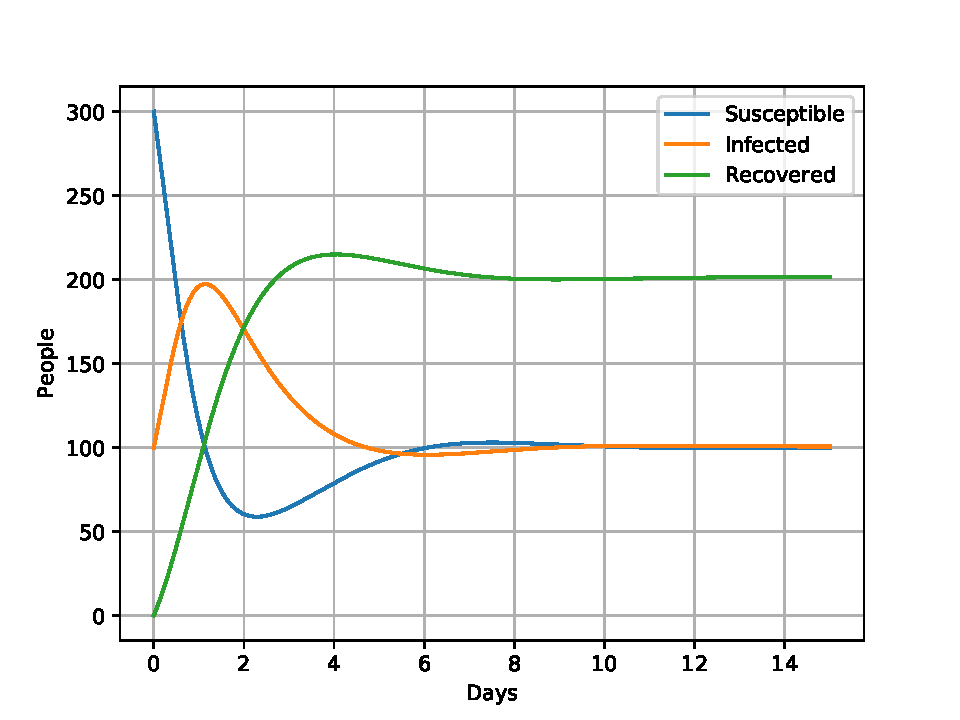
\includegraphics[scale=0.6]{../plots/opp_a_A.pdf}
		\caption{figure caption goes here}\label{fig:opp_a_A}
	\end{minipage}
	\begin{minipage}{0.49\textwidth}
		\centering
		\captionsetup{type=table} %% tell latex to change to table
		\begin{tabular}{|l|l|l|l|}
			\hline
			Group & Expected & Analytical   & Number  \\ \hline
			$s*$ & 0.25 & 0.2499 & 100.0 \\ \hline
			$i*$ & 0.25 & 0.2516 & 100.6 \\ \hline
			$r*$ & 0.5  & 0.5035 & 201.4 \\ \hline
		\end{tabular}
		\caption{table caption goes  here}\label{tab:opp_a_A}
	\end{minipage}
%	\caption{stuff}
\end{figure}

\begin{figure}
	\centering
	\begin{minipage}{0.49\textwidth}
		\centering
		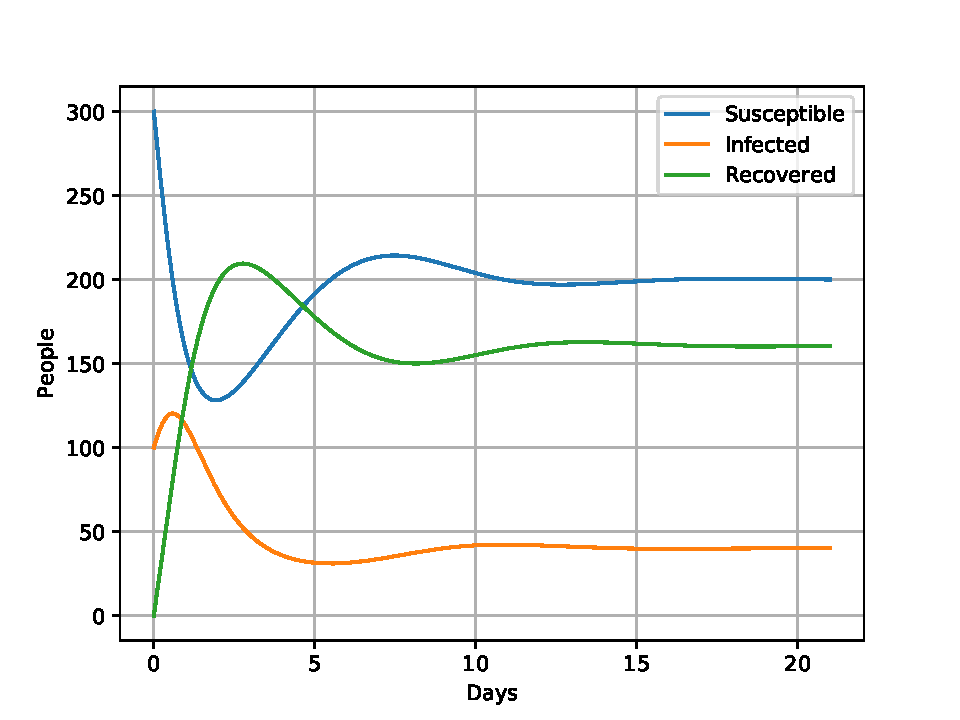
\includegraphics[scale=0.6]{../plots/opp_a_B.pdf}
		\caption{figure caption goes here}\label{fig:opp_a_B}
	\end{minipage}
	\begin{minipage}{0.49\textwidth}
		\centering
		\captionsetup{type=table} %% tell latex to change to table
		\begin{tabular}{|l|l|l|l|}
			\hline
			Group & Expected & Analytical   & Number  \\ \hline
			$s*$ & 0.5 & 0.5001 & 200.1 \\ \hline
			$i*$ & 0.1 & 0.1006 & 40.2 \\ \hline
			$r*$ & 0.4 & 0.4011 & 160.5 \\ \hline
		\end{tabular}
		\caption{table caption goes  here}\label{tab:opp_a_B}
	\end{minipage}
	%	\caption{stuff}
\end{figure}

\begin{figure}
	\centering
	\begin{minipage}{0.49\textwidth}
		\centering
		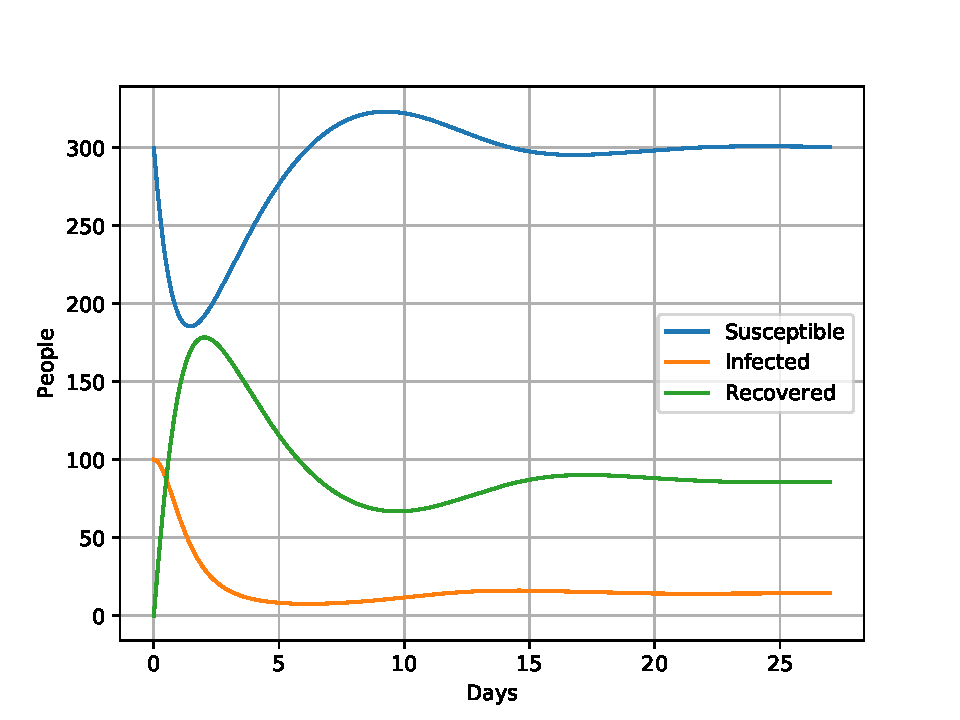
\includegraphics[scale=0.6]{../plots/opp_a_C.pdf}
		\caption{figure caption goes here}\label{fig:opp_a_C}
	\end{minipage}
	\begin{minipage}{0.49\textwidth}
		\centering
		\captionsetup{type=table} %% tell latex to change to table
		\begin{tabular}{|l|l|l|l|}
			\hline
			Group & Expected & Analytical   & Number  \\ \hline
			$s*$ & 0.75 & 0.7511 & 300.5 \\ \hline
			$i*$ & 0.0357 & 0.0360 & 14.4 \\ \hline
			$r*$ & 0.2143 & 0.2145 & 85.8 \\ \hline
		\end{tabular}
		\caption{table caption goes  here}\label{tab:opp_a_C}
	\end{minipage}
	%	\caption{stuff}
\end{figure}

\begin{figure}
	\centering
	\begin{minipage}{0.49\textwidth}
		\centering
		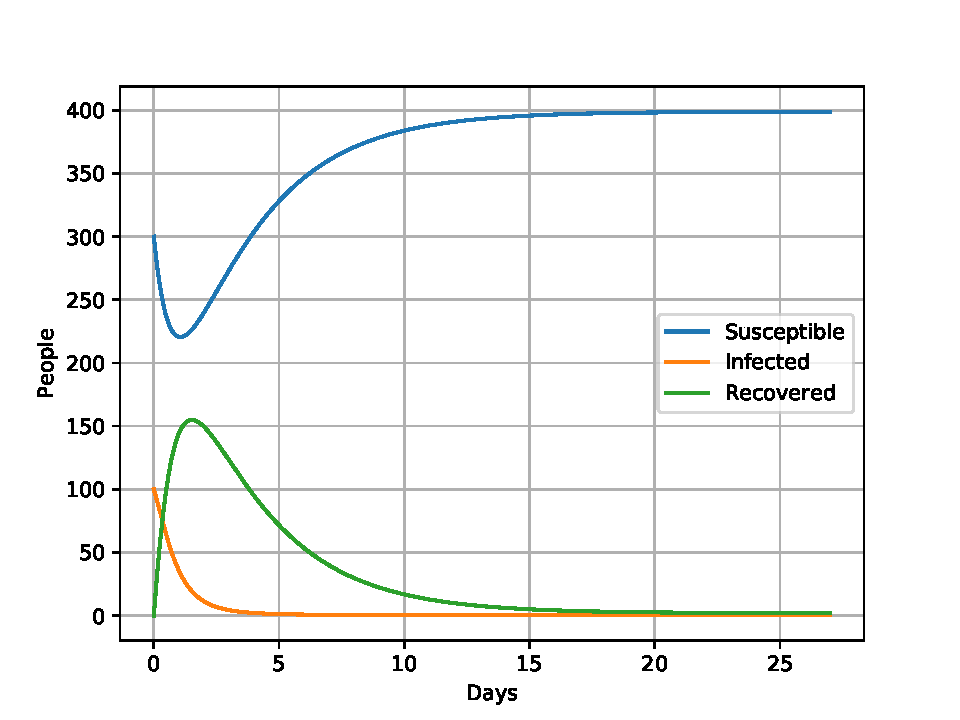
\includegraphics[scale=0.6]{../plots/opp_a_D.pdf}
		\caption{figure caption goes here}\label{fig:opp_a_D}
	\end{minipage}
	\begin{minipage}{0.49\textwidth}
		\centering
		\captionsetup{type=table} %% tell latex to change to table
		\begin{tabular}{|l|l|l|l|}
			\hline
			Group & Expected & Analytical   & Number  \\ \hline
			$s*$ & 1.0 & 0.9974 & 399.0 \\ \hline
			$i*$ & 0.0 & 0.0006 & 0.2 \\ \hline
			$r*$ & 0.0 & 0.0047 & 1.9 \\ \hline
		\end{tabular}
		\caption{table caption goes  here}\label{tab:opp_a_D}
	\end{minipage}
	%	\caption{stuff}
\end{figure}

\begin{figure}
	\centering
	\begin{minipage}{0.49\textwidth}
		\centering
		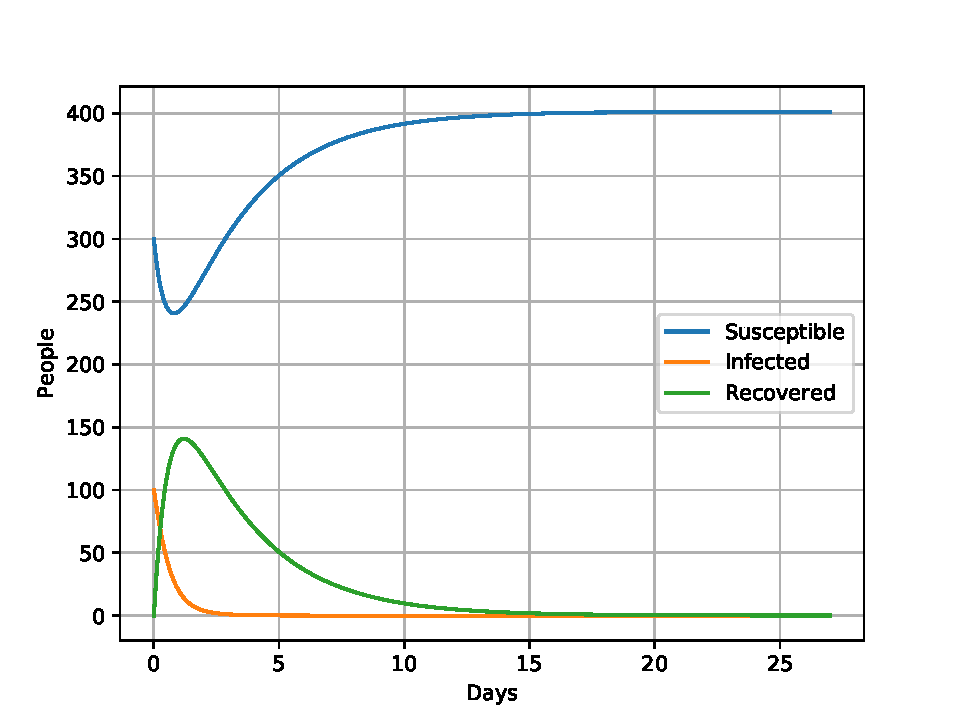
\includegraphics[scale=0.6]{../plots/opp_a_E.pdf}
		\caption{figure caption goes here}\label{fig:opp_a_E}
	\end{minipage}
	\begin{minipage}{0.49\textwidth}
		\centering
		\captionsetup{type=table} %% tell latex to change to table
		\begin{tabular}{|l|l|l|l|}
			\hline
			Group & Expected & Analytical   & Number  \\ \hline
			$s*$ & 1.25 & 1.0034 & 401.4 \\ \hline
			$i*$ & -0.0227 & $4.7119\cdot 10^{-11}$ & $1.9\cdot 10^{-8}$ \\ \hline
			$r*$ & -0.2273 & $8.4064\cdot 10^{-5}$ & $3.4\cdot 10^{-2}$ \\ \hline
		\end{tabular}
		\caption{table caption goes  here}\label{tab:opp_a_E}
	\end{minipage}
	%	\caption{stuff}
\end{figure}


\subsection{Monte Carlo}


\subsection{Vital dynamics}

\begin{figure}[!htb]
	\centering 
	%Scale angir størrelsen på bildet. Bildefilen må ligge i samme mappe som tex-filen. 
	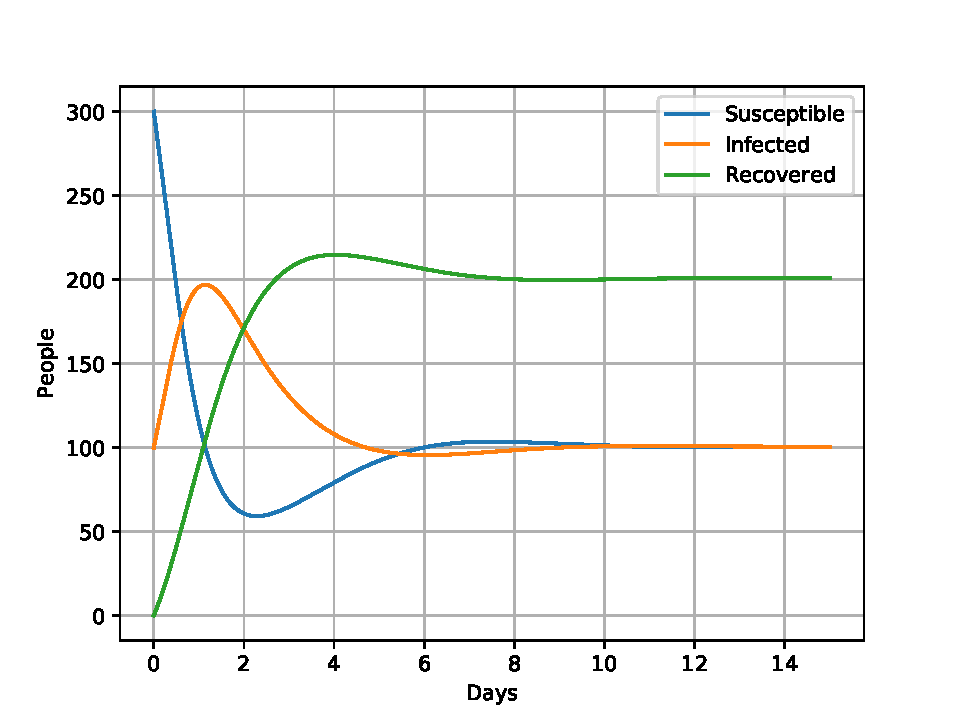
\includegraphics[scale=0.56]{../plots/opp_c_A0.pdf}
	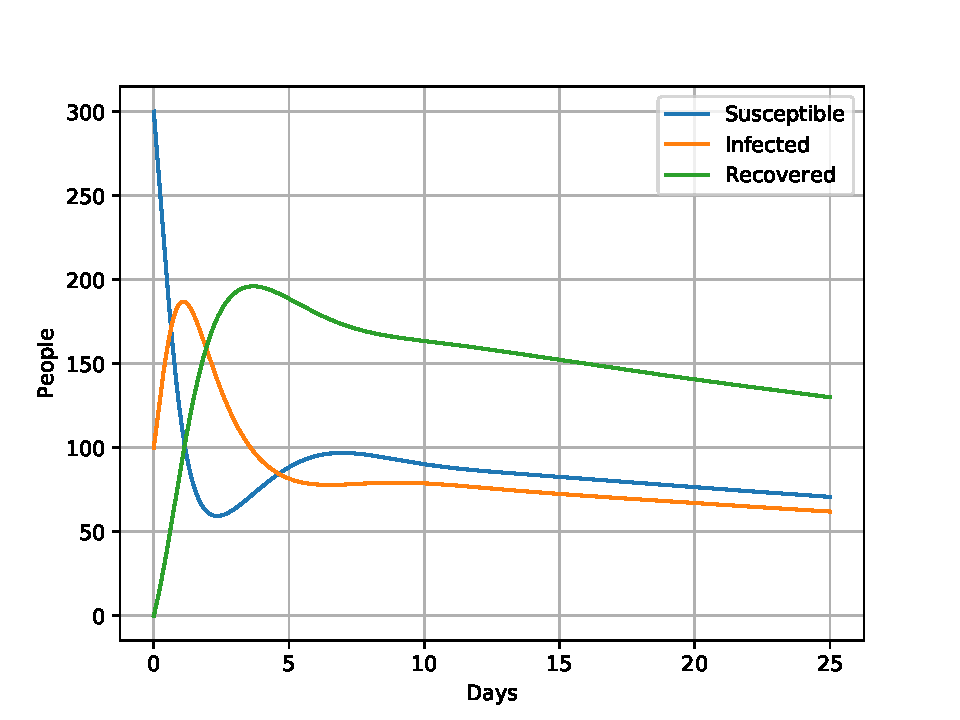
\includegraphics[scale=0.56]{../plots/opp_c_A1.pdf}
	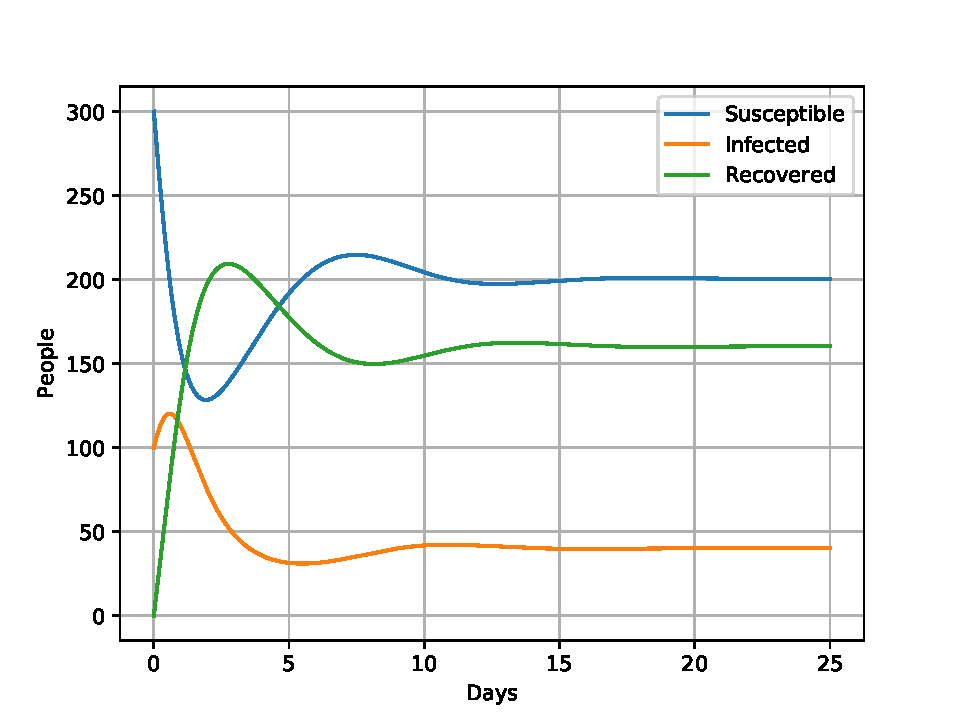
\includegraphics[scale=0.56]{../plots/opp_c_B0.pdf}
	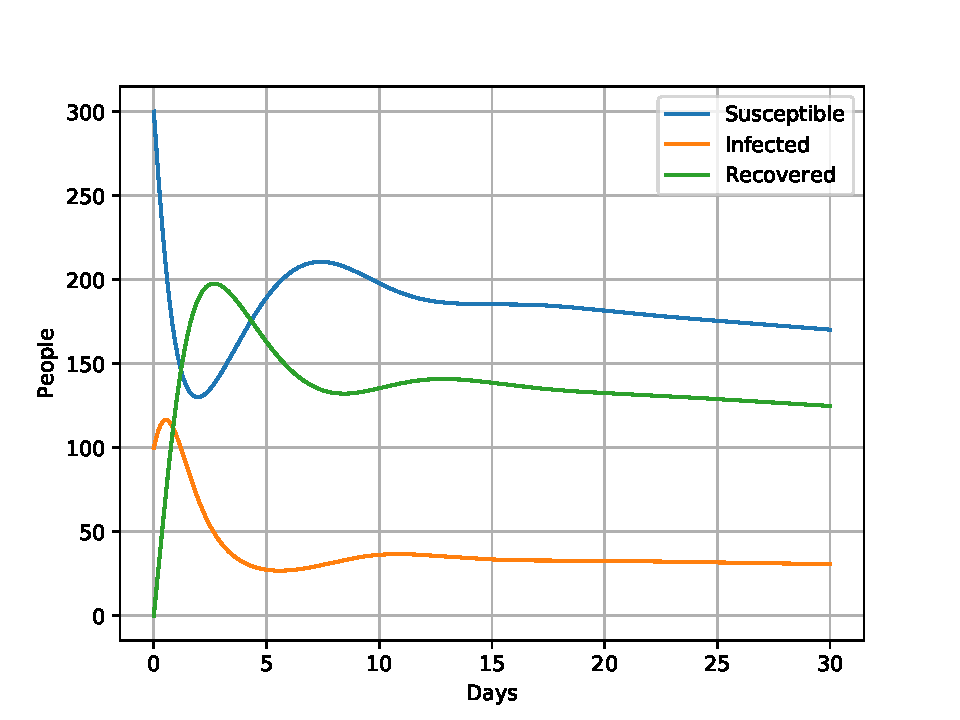
\includegraphics[scale=0.56]{../plots/opp_c_B1.pdf}	
	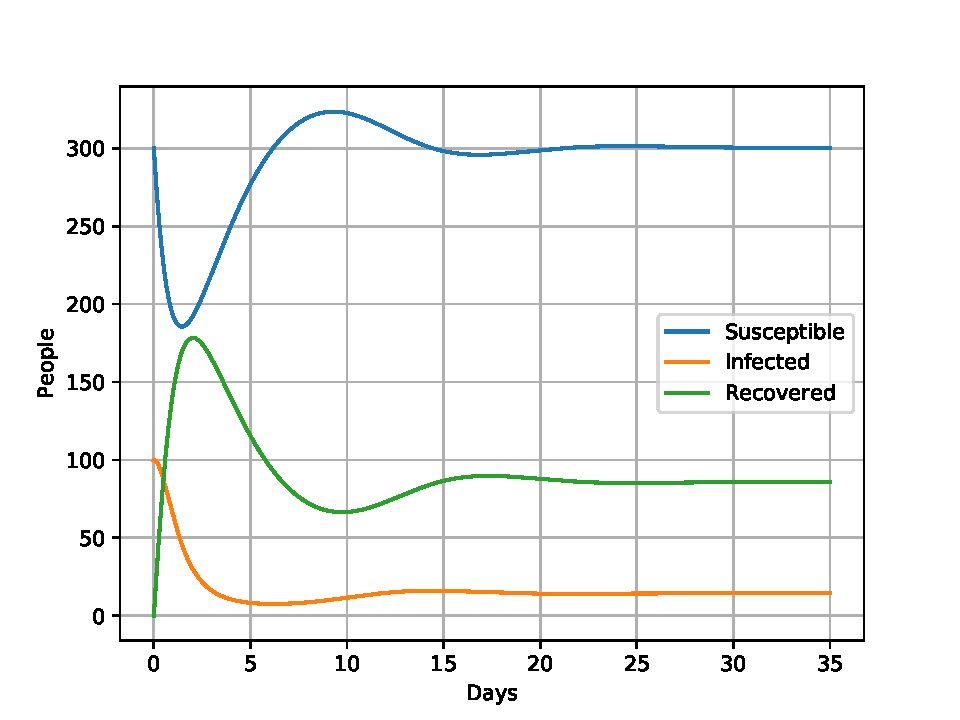
\includegraphics[scale=0.56]{../plots/opp_c_C0.pdf}
	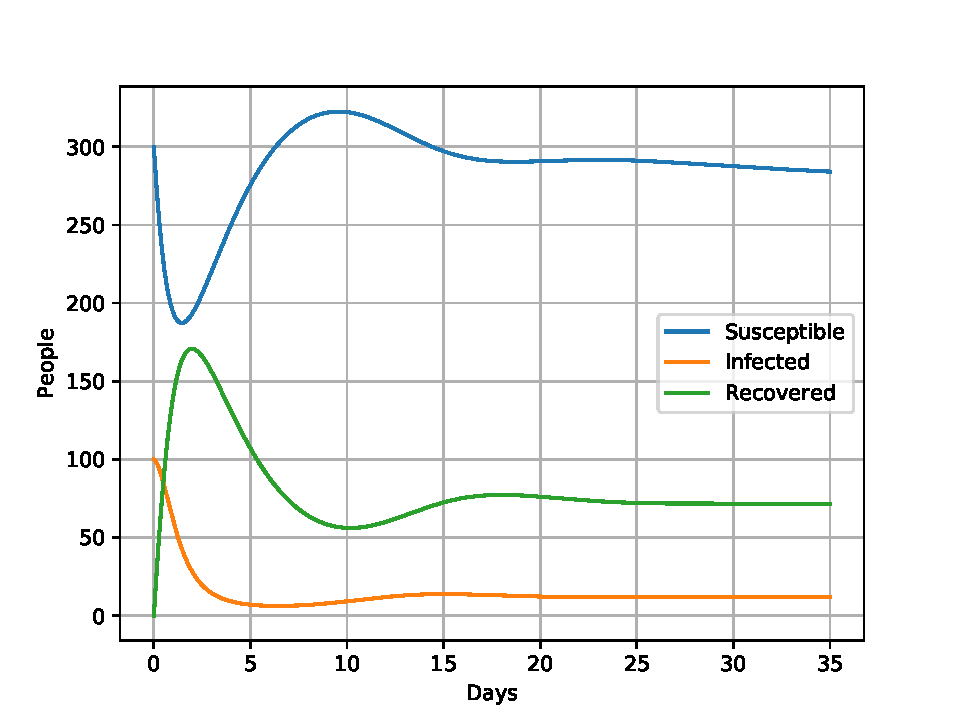
\includegraphics[scale=0.56]{../plots/opp_c_C1.pdf}
	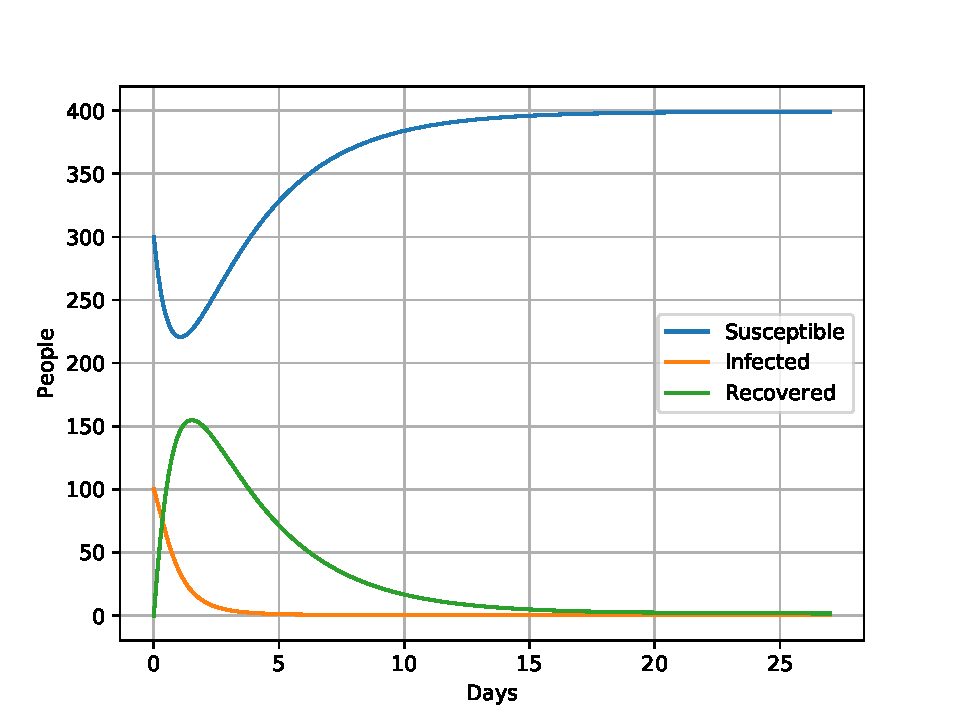
\includegraphics[scale=0.56]{../plots/opp_c_D0.pdf}
	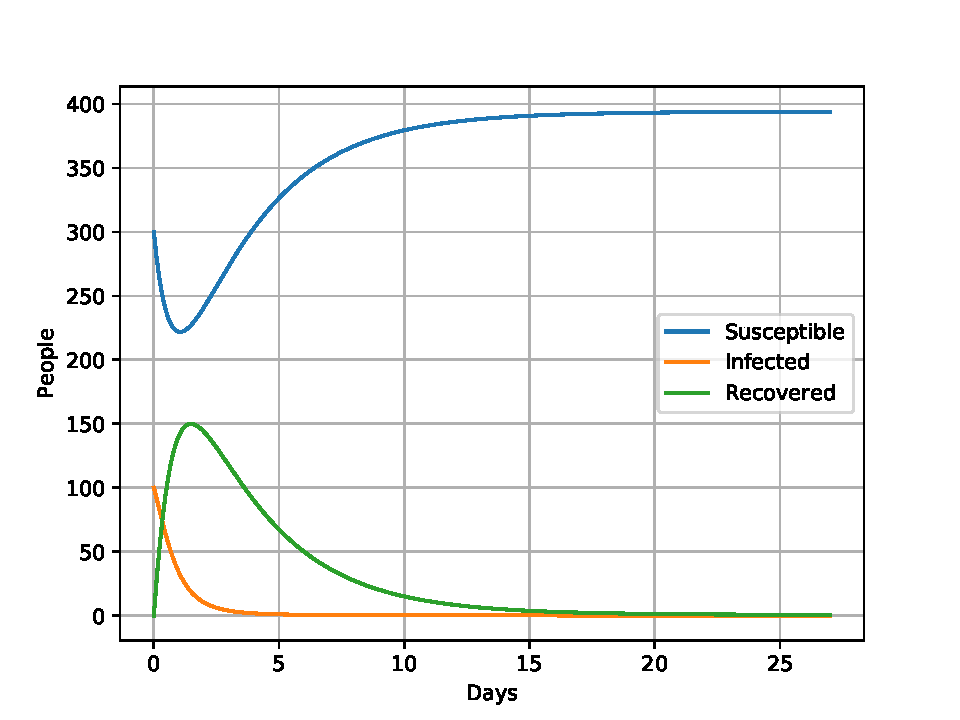
\includegraphics[scale=0.56]{../plots/opp_c_D1.pdf}	
	\caption{fyll inn}
	%Label gjør det enkelt å referere til ulike bilder.
	\label{opp_c0}
\end{figure}

\begin{figure}[!htb]
	\centering 
	%Scale angir størrelsen på bildet. Bildefilen må ligge i samme mappe som tex-filen. 
	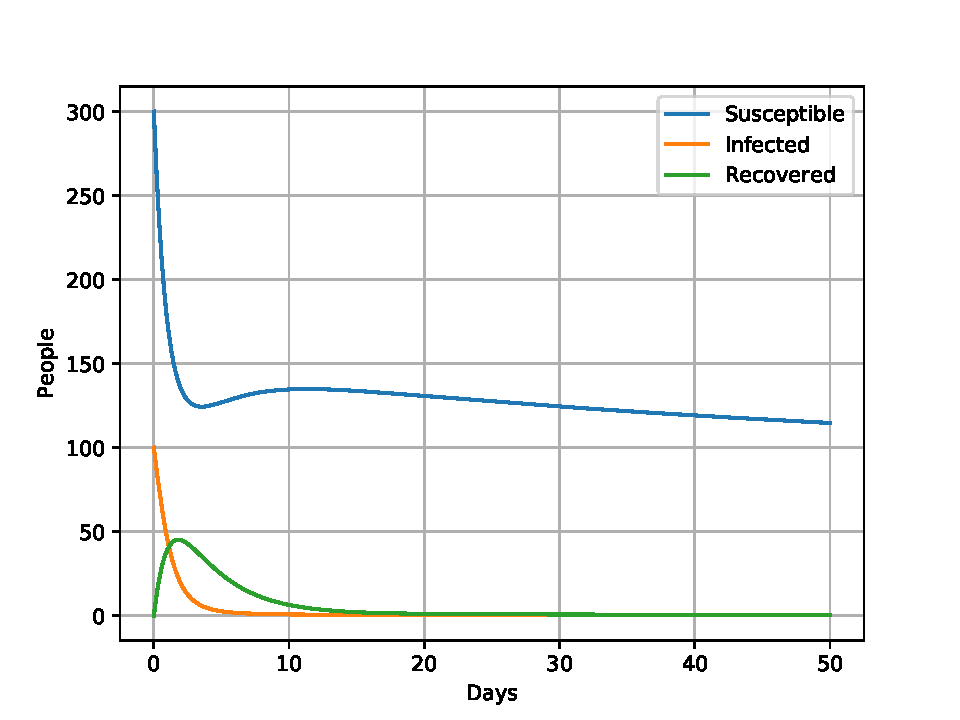
\includegraphics[scale=0.56]{../plots/opp_c_k0.pdf}
	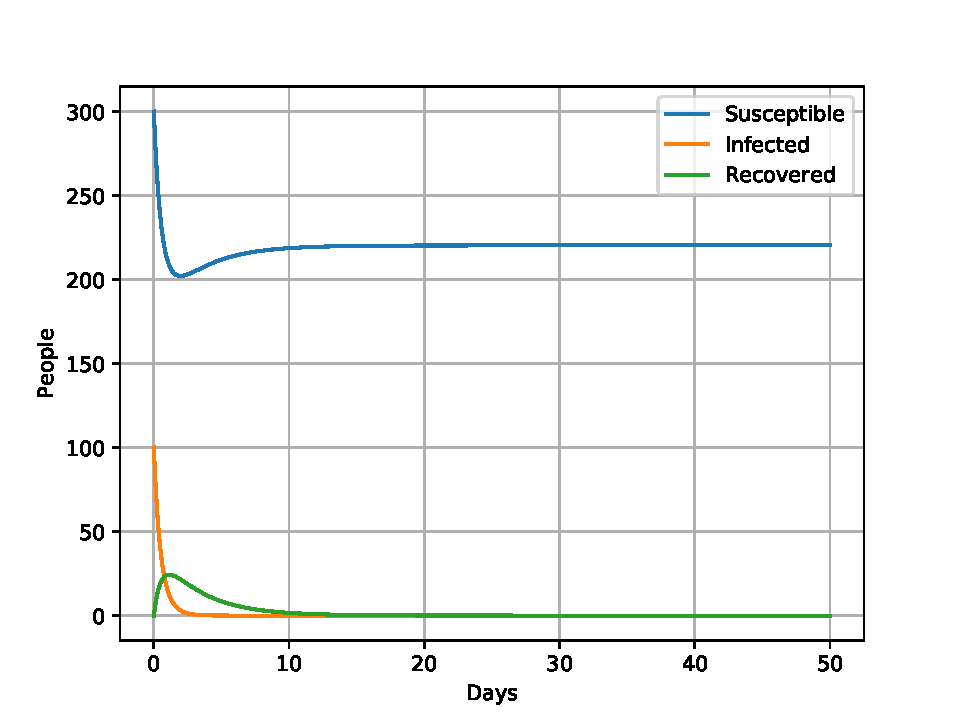
\includegraphics[scale=0.56]{../plots/opp_c_k1.pdf}
	%trenger kansjke ikke begge disse
	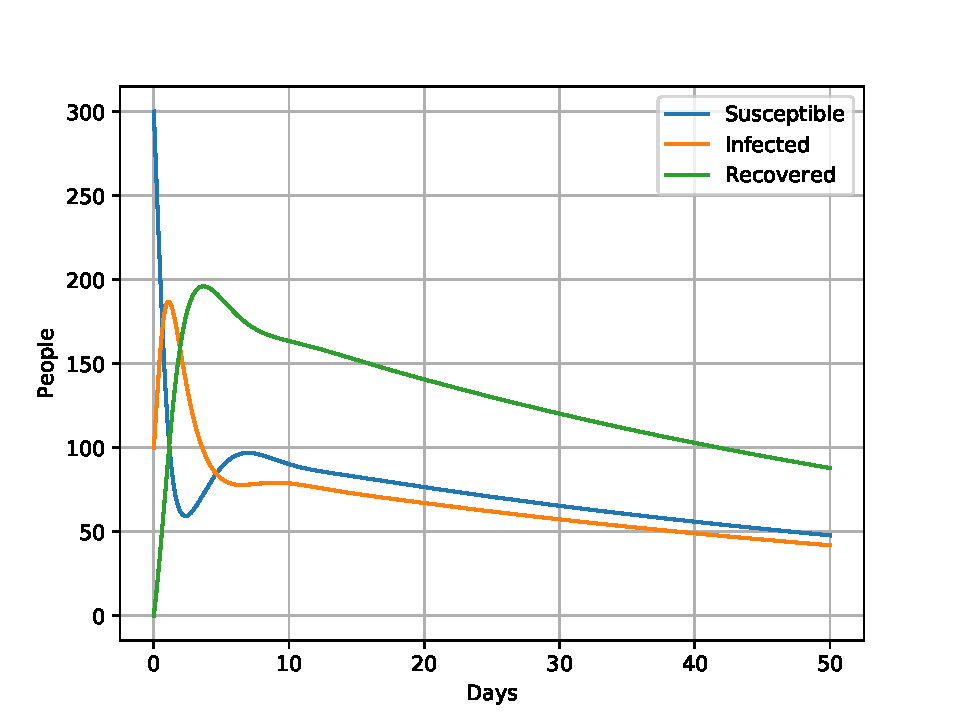
\includegraphics[scale=0.56]{../plots/opp_c_k2.pdf}
	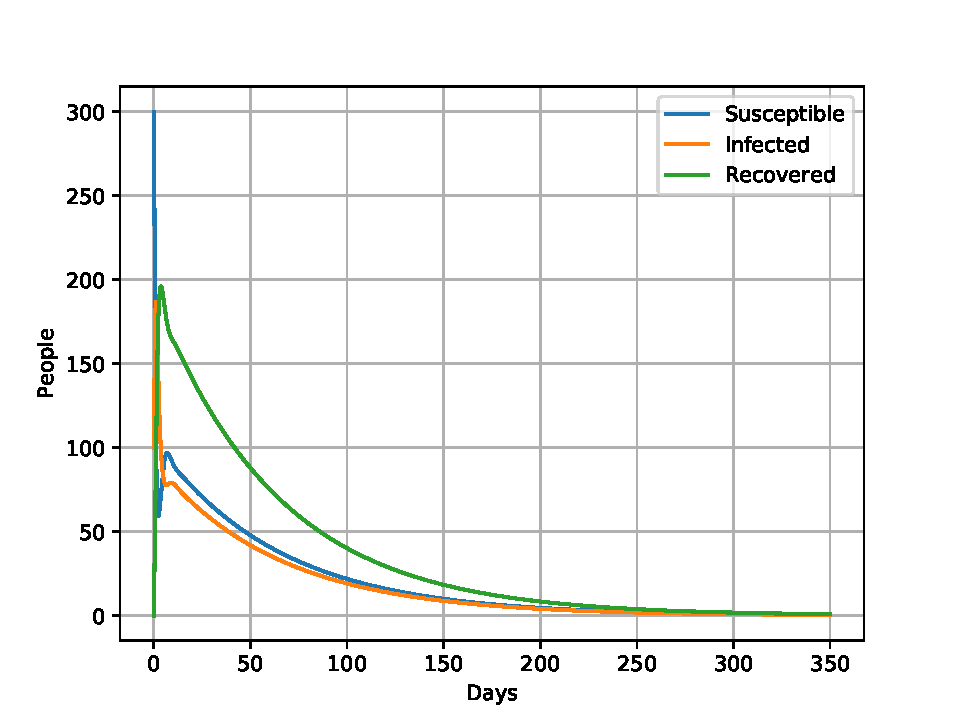
\includegraphics[scale=0.56]{../plots/opp_c_k2l.pdf}	
	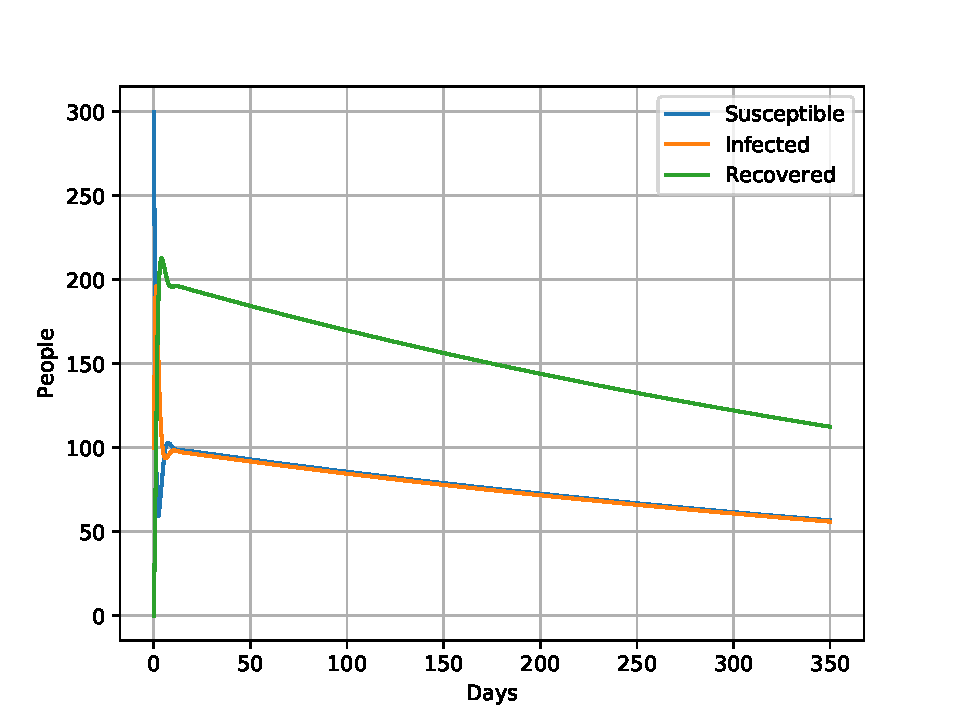
\includegraphics[scale=0.56]{../plots/opp_c_k3.pdf} %kan kaskje være først?
	%mulig jeg bør splitte denne
	\caption{fyll inn}
	%Label gjør det enkelt å referere til ulike bilder.
	\label{opp_c1}
\end{figure}

\begin{figure}[!htb]
	\centering 
	%Scale angir størrelsen på bildet. Bildefilen må ligge i samme mappe som tex-filen. 
	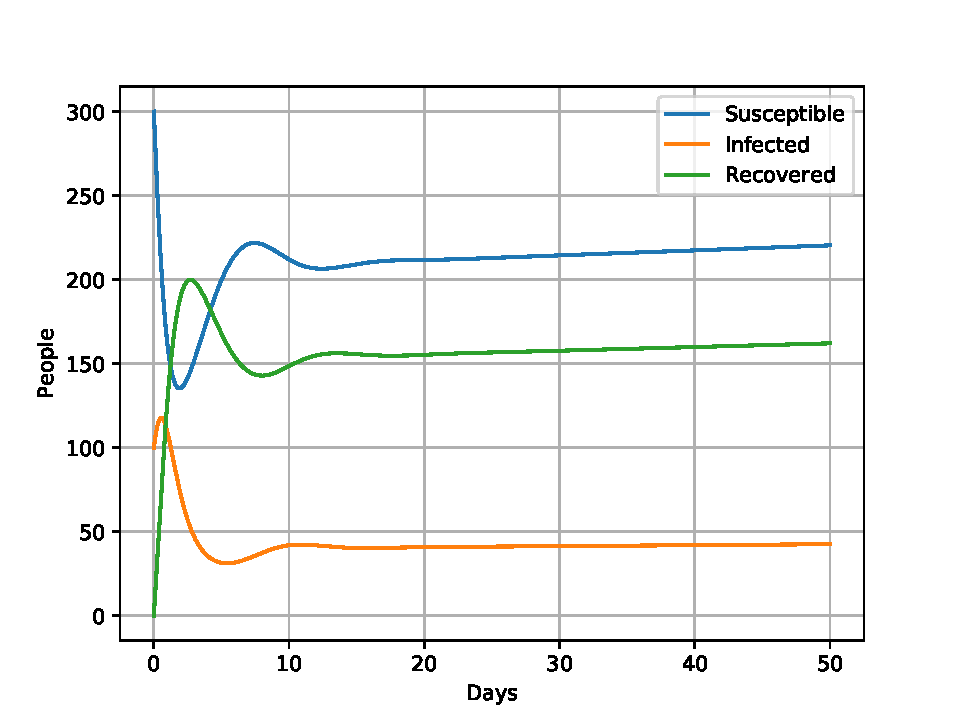
\includegraphics[scale=0.56]{../plots/opp_c_h_10000.pdf}
	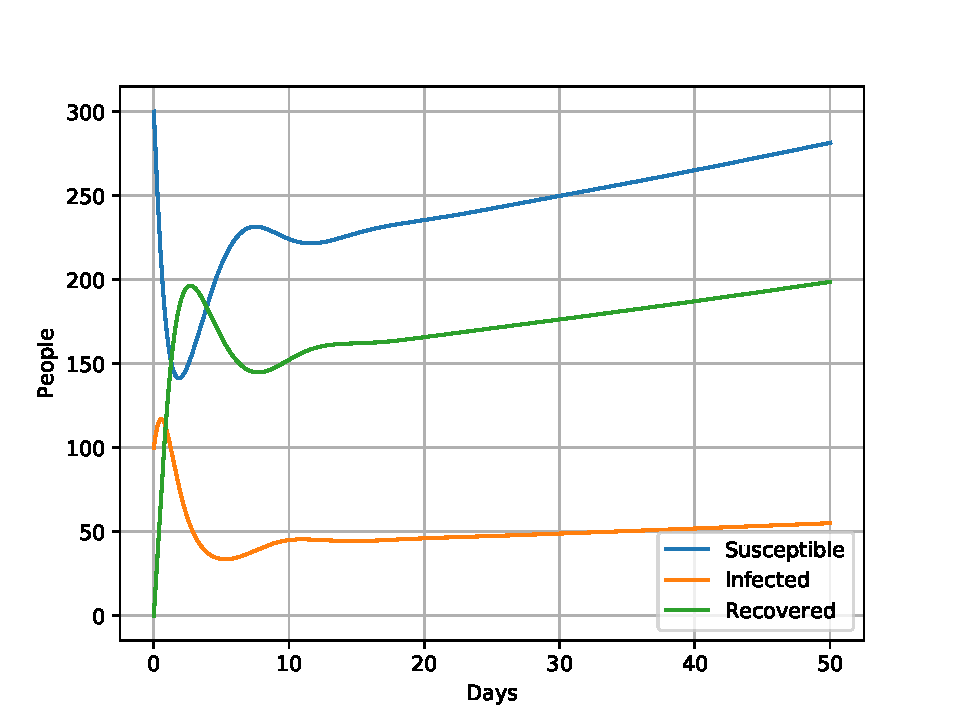
\includegraphics[scale=0.56]{../plots/opp_c_h_20000.pdf}	
	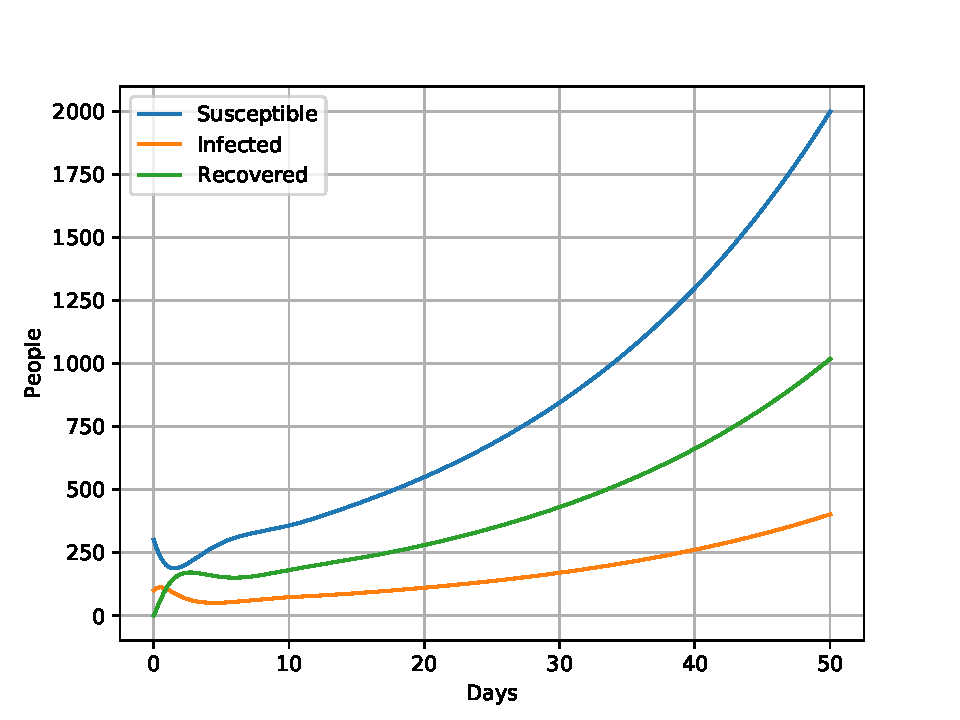
\includegraphics[scale=0.56]{../plots/opp_c_h_100000.pdf}
	\caption{fyll inn}
	%Label gjør det enkelt å referere til ulike bilder.
	\label{opp_c2}
\end{figure}


\subsection{Seasonal Variation}

\begin{figure}[!htb]
	\centering 
	%Scale angir størrelsen på bildet. Bildefilen må ligge i samme mappe som tex-filen. 
	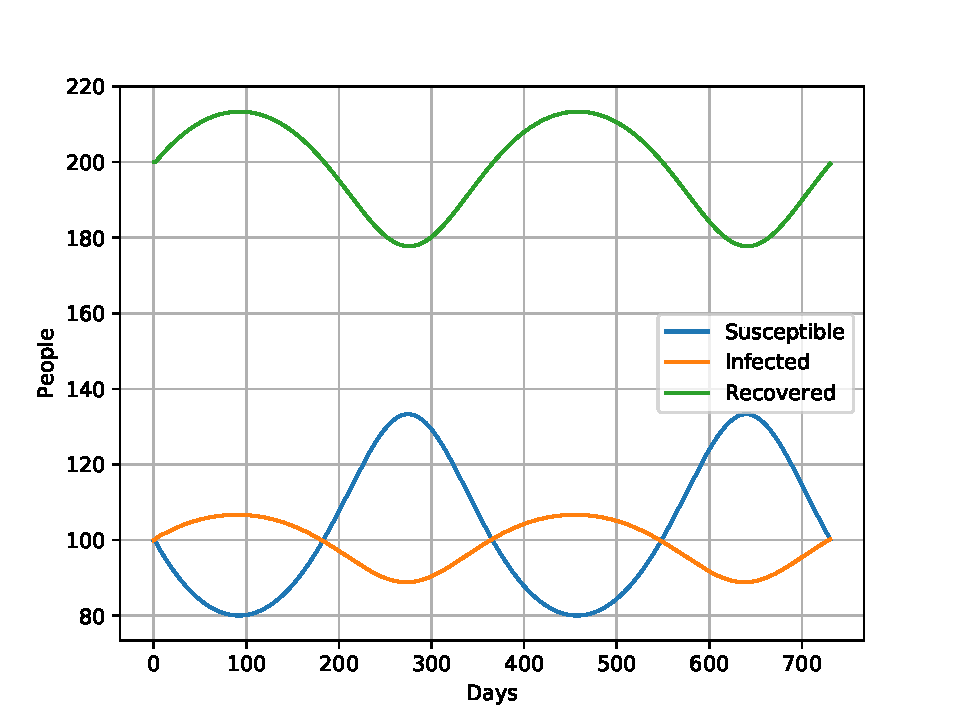
\includegraphics[scale=0.56]{../plots/opp_d_A.pdf}
	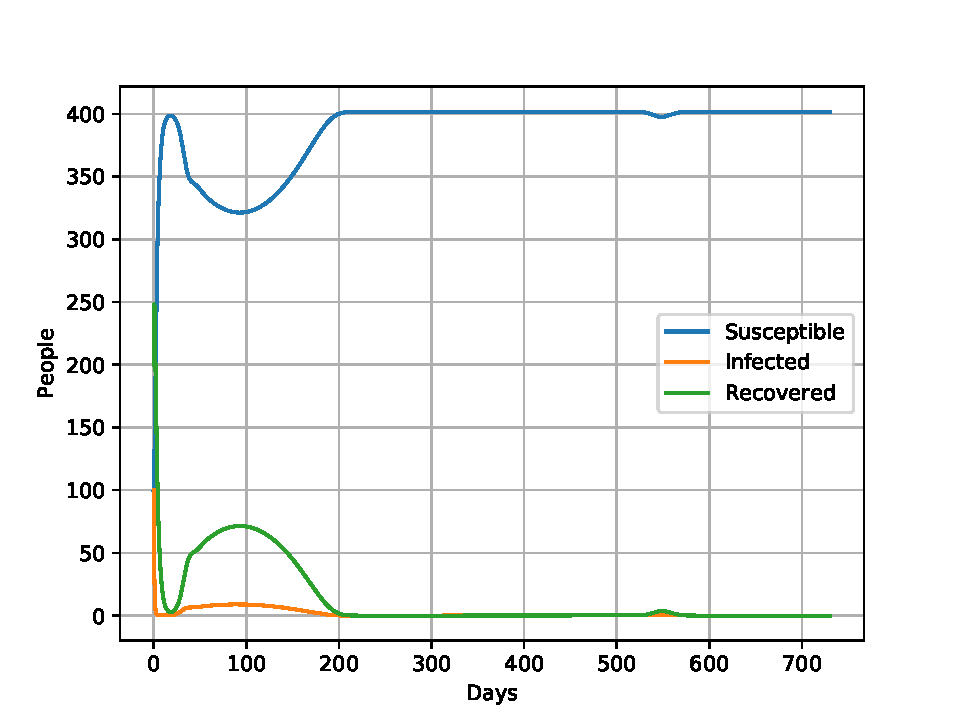
\includegraphics[scale=0.56]{../plots/opp_d_B.pdf}	
	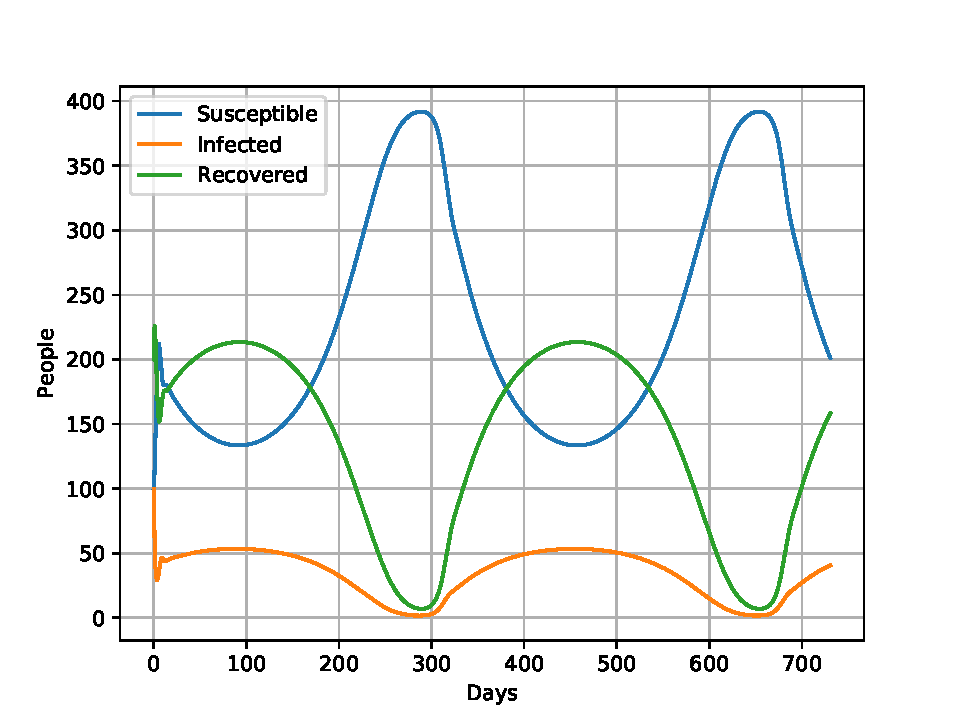
\includegraphics[scale=0.56]{../plots/opp_d_C.pdf}
	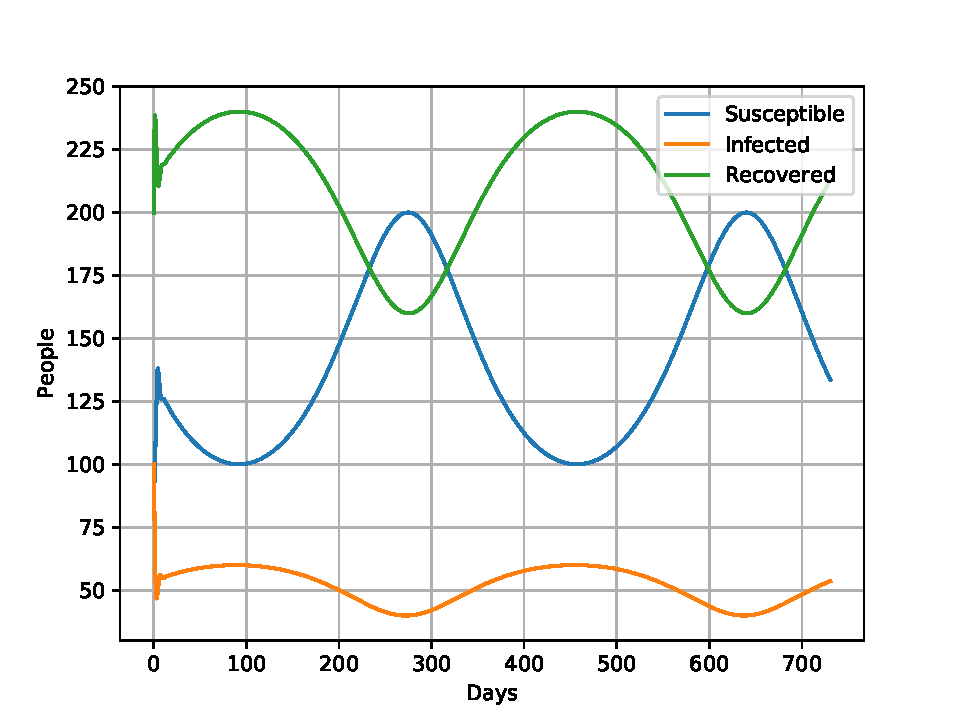
\includegraphics[scale=0.56]{../plots/opp_d_D.pdf}
	\caption{fyll inn}
	%Label gjør det enkelt å referere til ulike bilder.
	\label{opp_d0}
\end{figure}


\subsection{Vaccination}

\begin{figure}[!htb]
	\centering 
	%Scale angir størrelsen på bildet. Bildefilen må ligge i samme mappe som tex-filen. 
	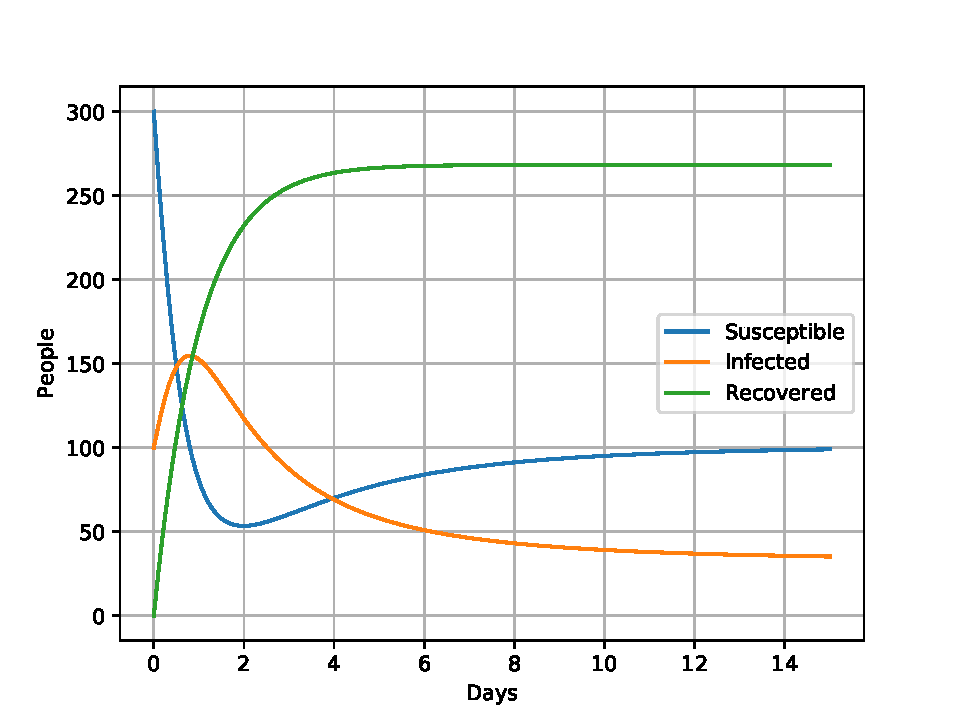
\includegraphics[scale=0.56]{../plots/opp_e_A0.pdf}
	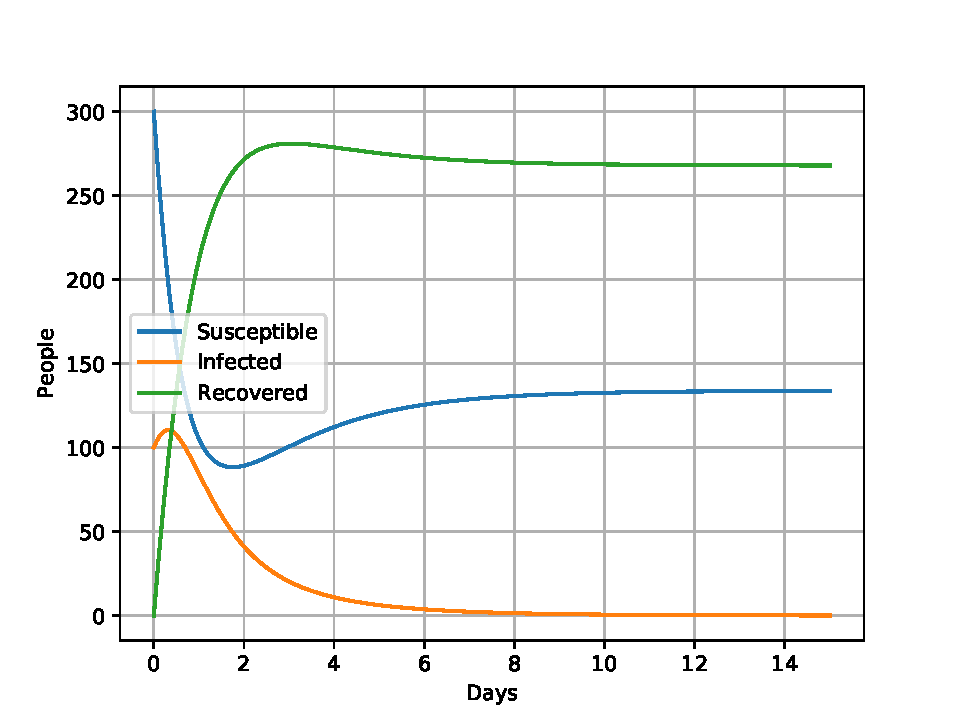
\includegraphics[scale=0.56]{../plots/opp_e_B0.pdf}	
	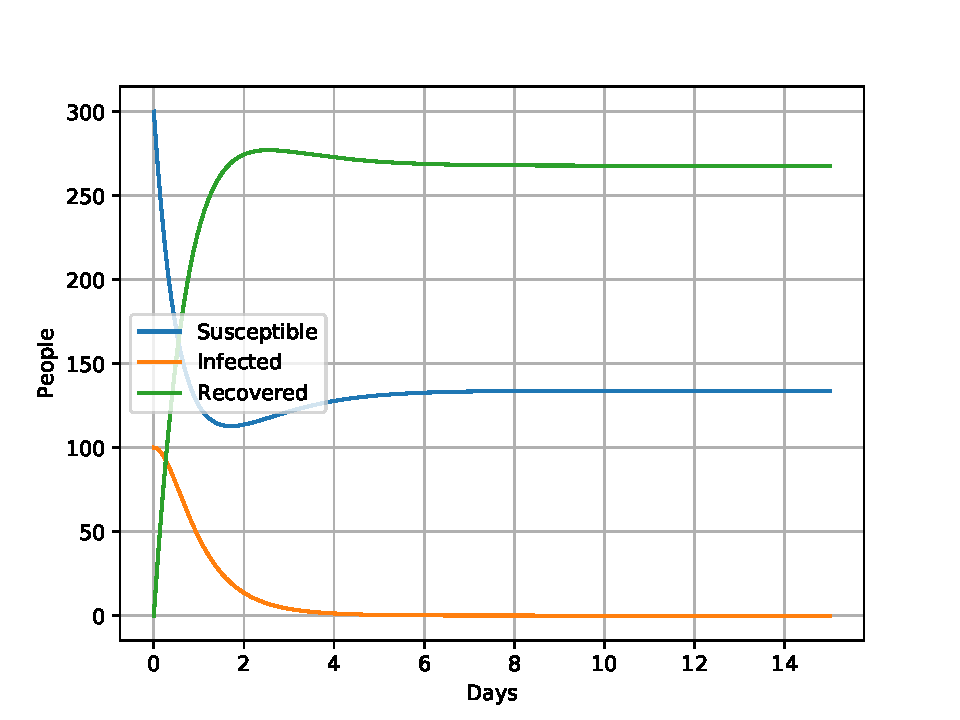
\includegraphics[scale=0.56]{../plots/opp_e_C0.pdf}
	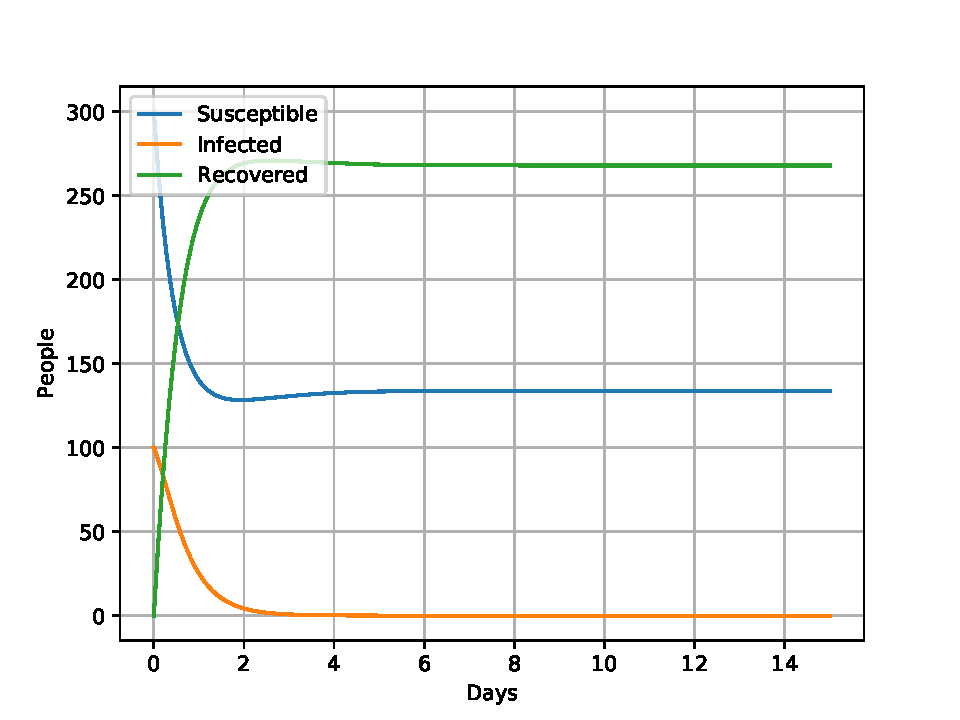
\includegraphics[scale=0.56]{../plots/opp_e_D0.pdf}
	\caption{fyll inn}
	%Label gjør det enkelt å referere til ulike bilder.
	\label{opp_e0}
\end{figure}

\begin{figure}[!htb]
	\centering 
	%Scale angir størrelsen på bildet. Bildefilen må ligge i samme mappe som tex-filen. 
	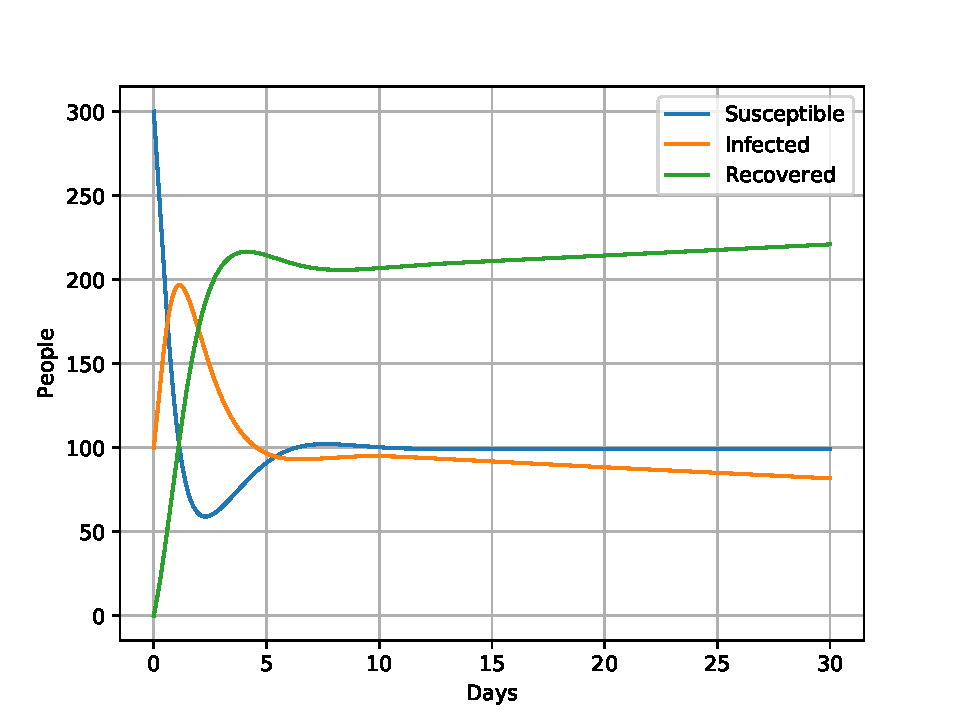
\includegraphics[scale=0.56]{../plots/opp_e_A1.pdf}
	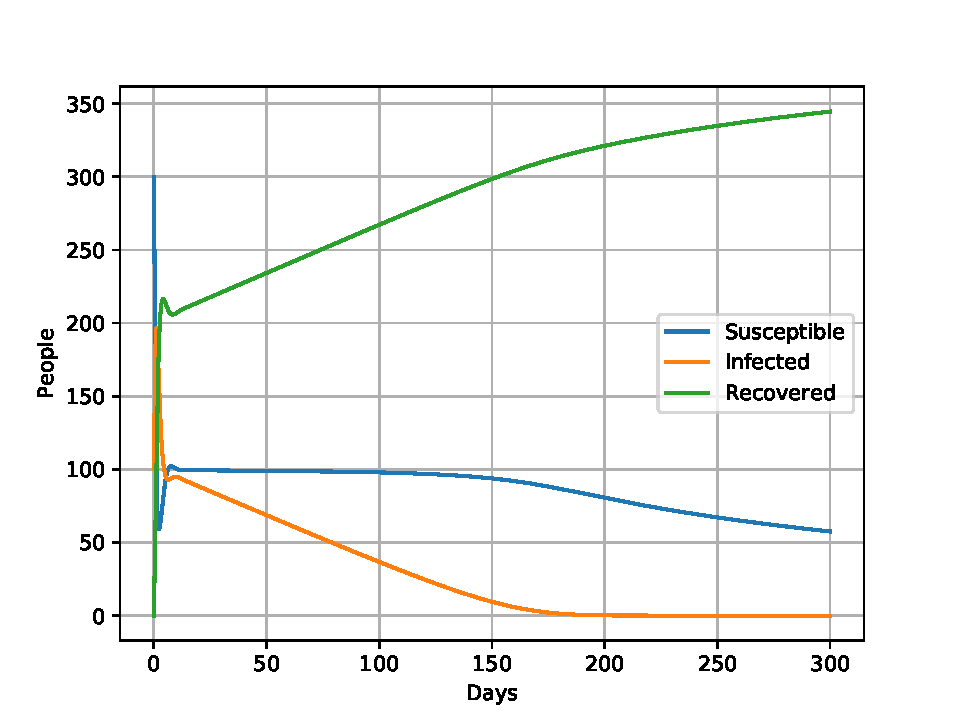
\includegraphics[scale=0.56]{../plots/opp_e_A2.pdf}
%	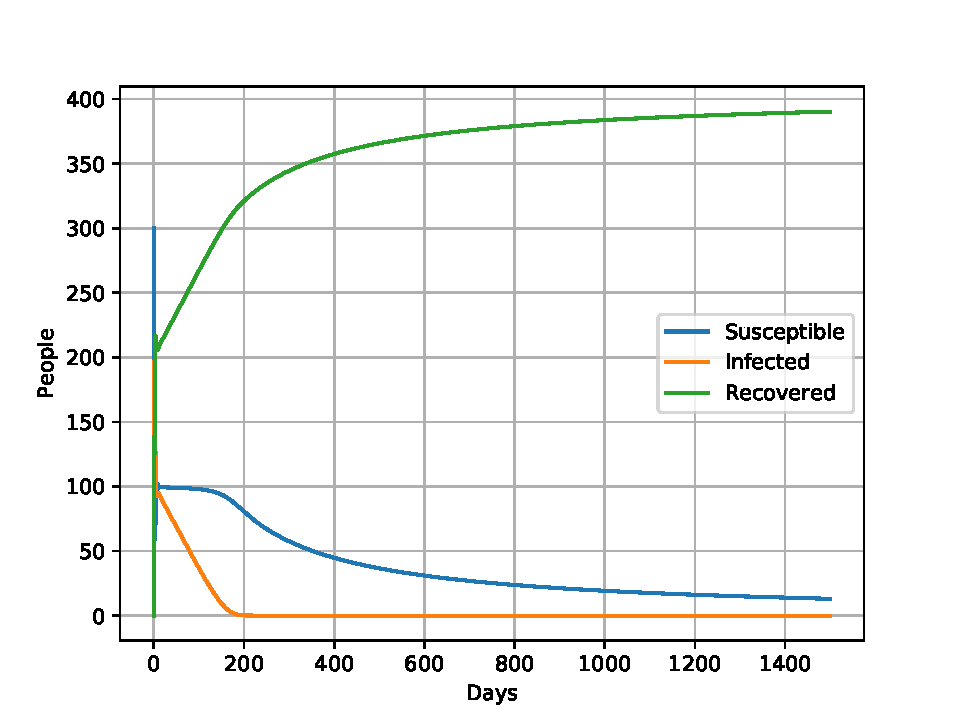
\includegraphics[scale=0.56]{../plots/opp_e_A3.pdf}
	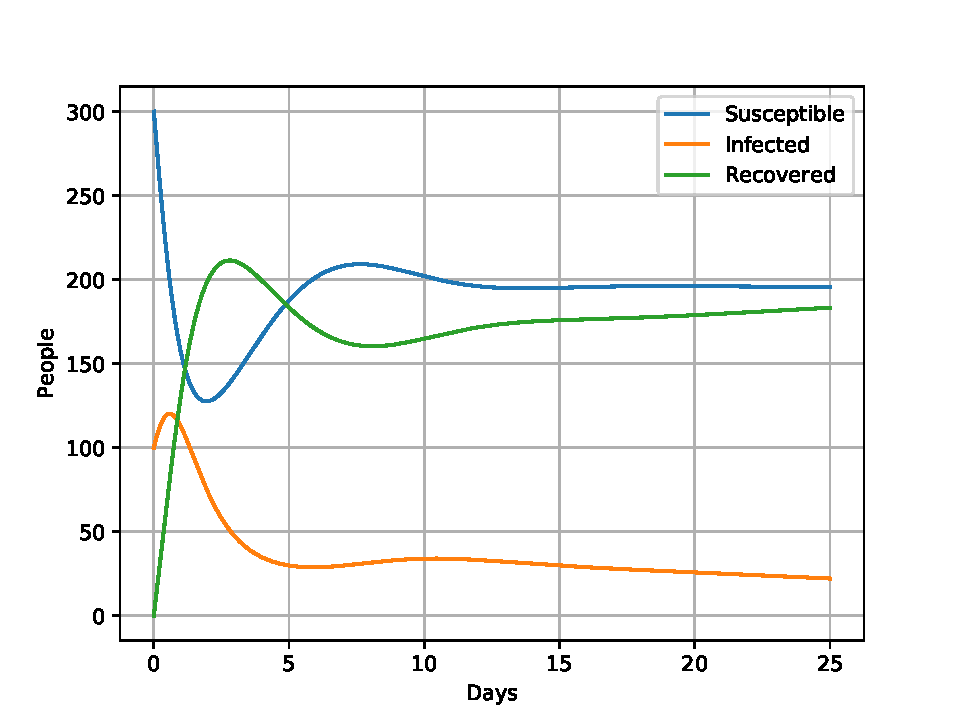
\includegraphics[scale=0.56]{../plots/opp_e_B1.pdf}	
	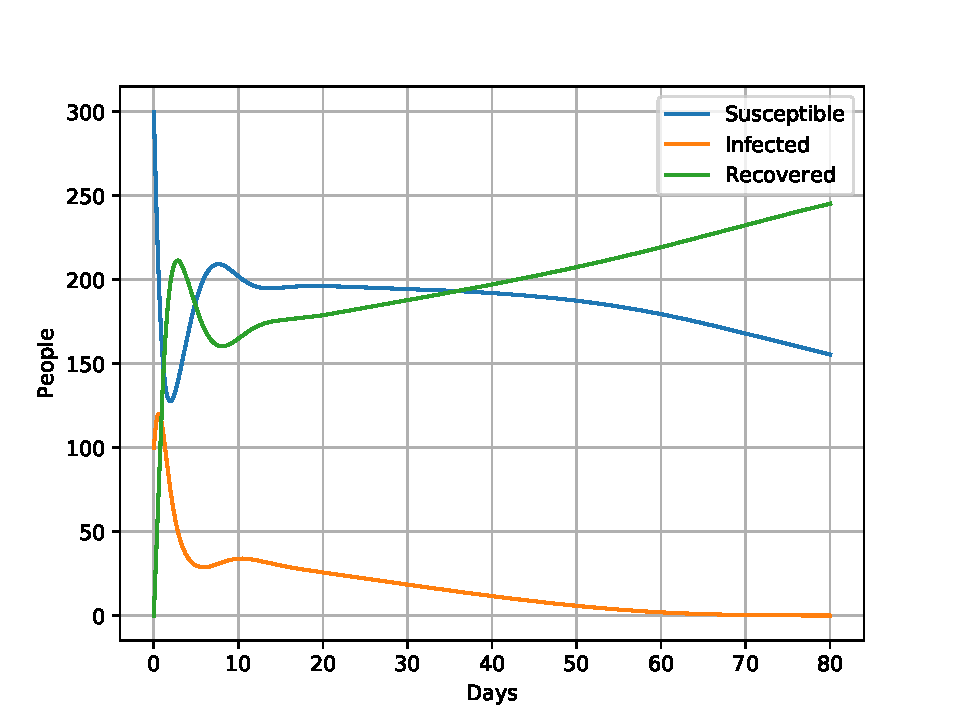
\includegraphics[scale=0.56]{../plots/opp_e_B2.pdf}	
	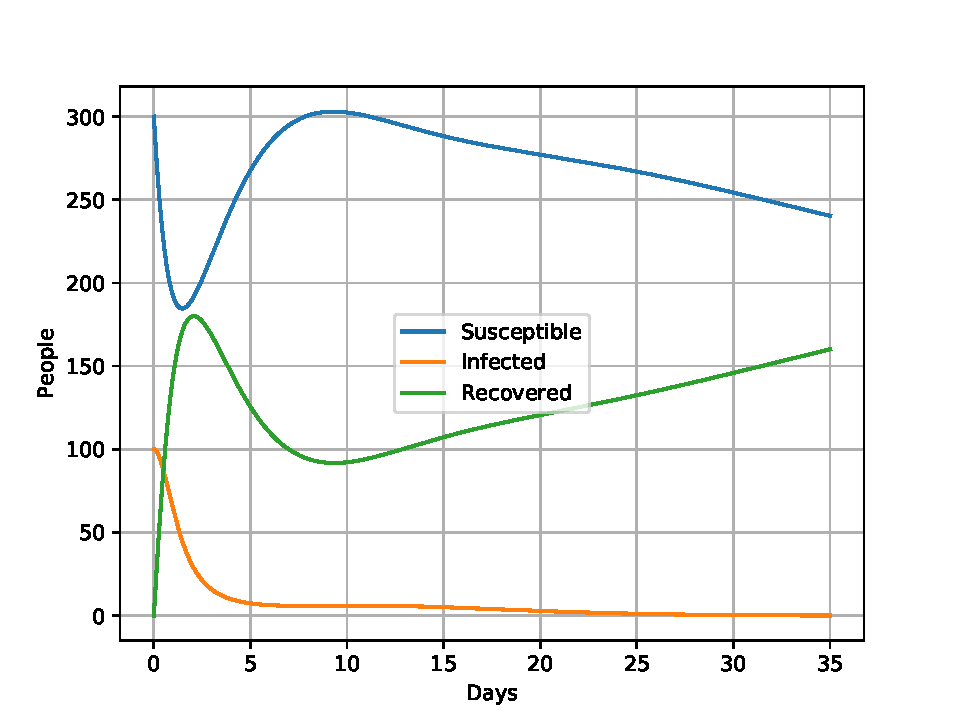
\includegraphics[scale=0.56]{../plots/opp_e_C1.pdf}
	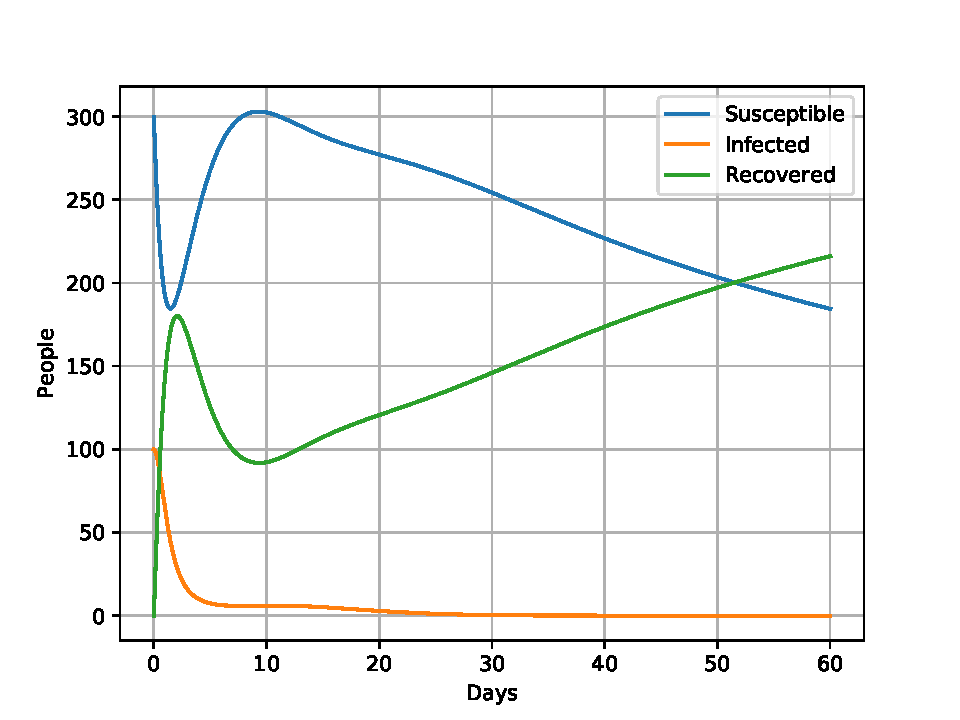
\includegraphics[scale=0.56]{../plots/opp_e_C2.pdf}
	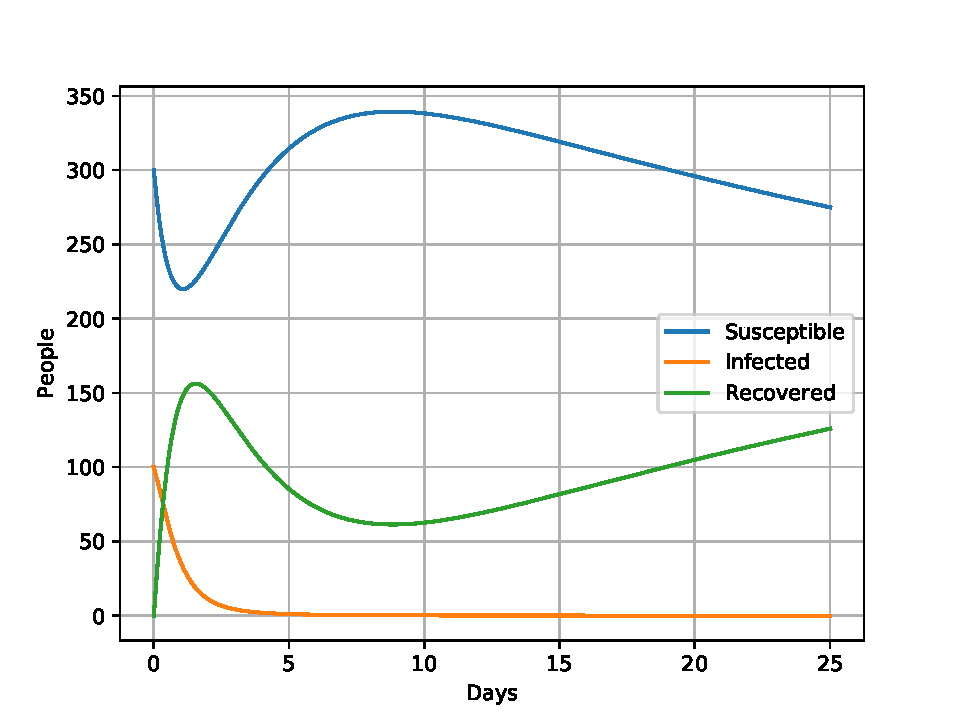
\includegraphics[scale=0.56]{../plots/opp_e_D1.pdf}
	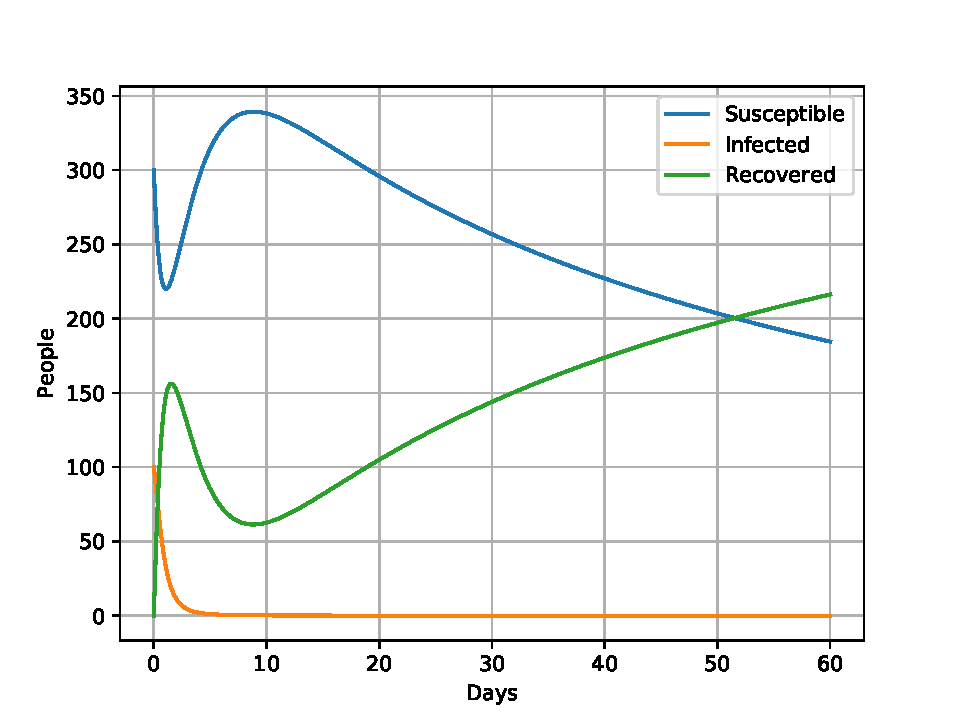
\includegraphics[scale=0.56]{../plots/opp_e_D2.pdf}
	\caption{fyll inn}
	%Label gjør det enkelt å referere til ulike bilder.
	\label{opp_e1}
\end{figure}

\begin{figure}[!htb]
	\centering 
	%Scale angir størrelsen på bildet. Bildefilen må ligge i samme mappe som tex-filen. 
	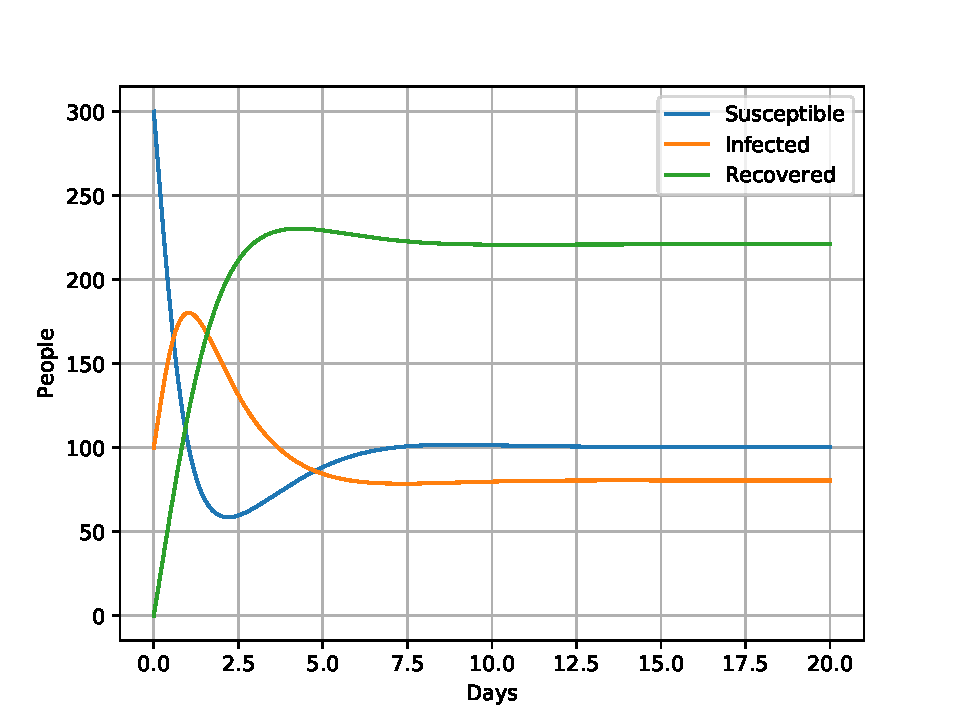
\includegraphics[scale=0.56]{../plots/opp_e_fa.pdf}
	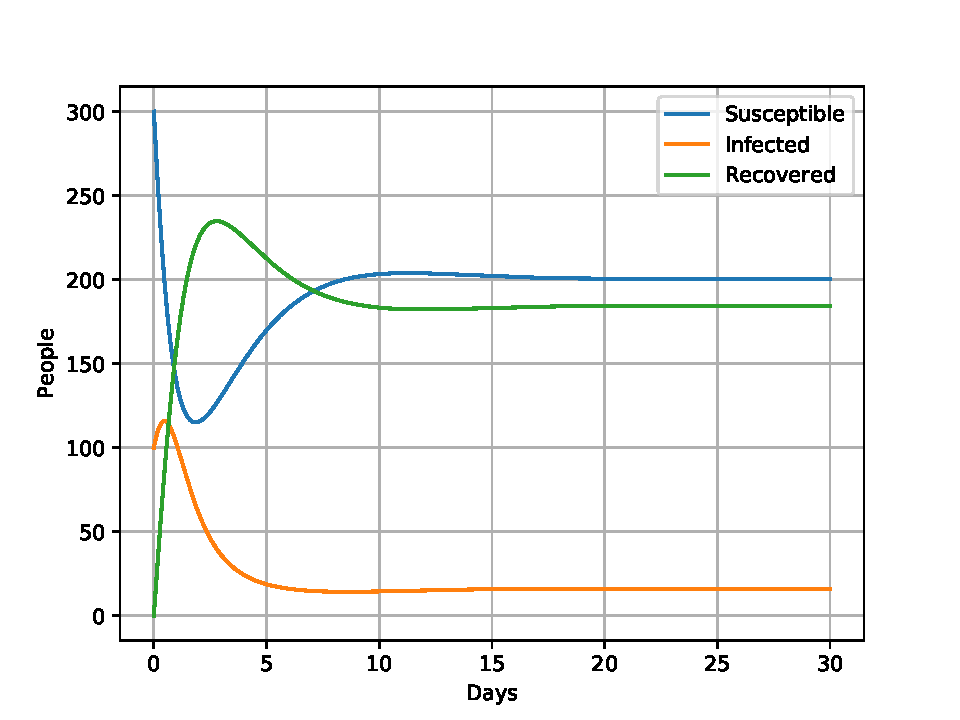
\includegraphics[scale=0.56]{../plots/opp_e_fb.pdf}	
	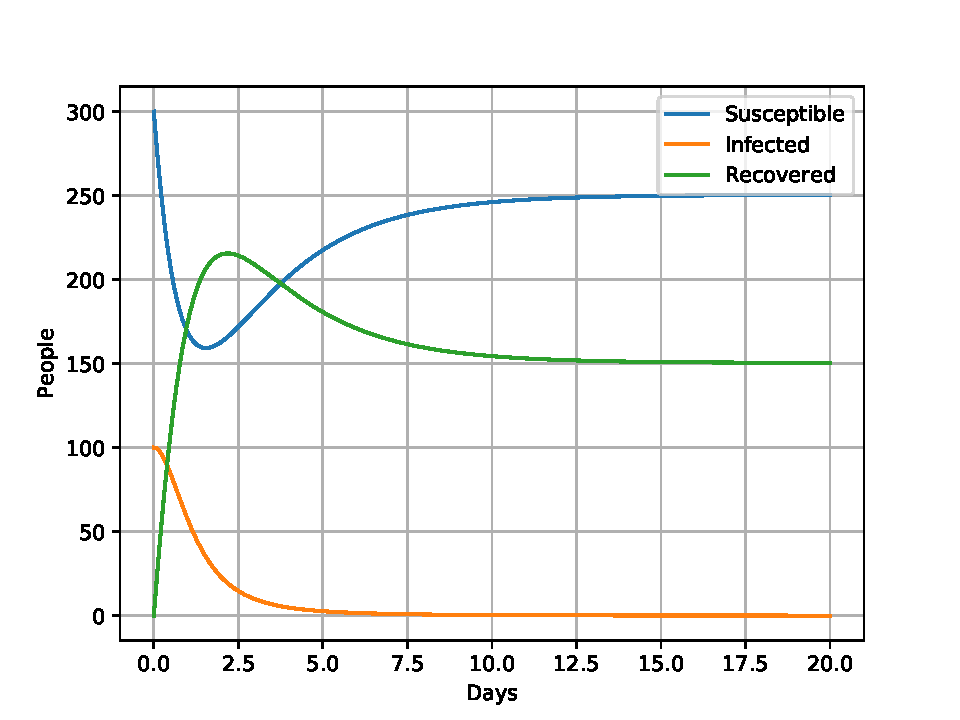
\includegraphics[scale=0.56]{../plots/opp_e_fc.pdf}
	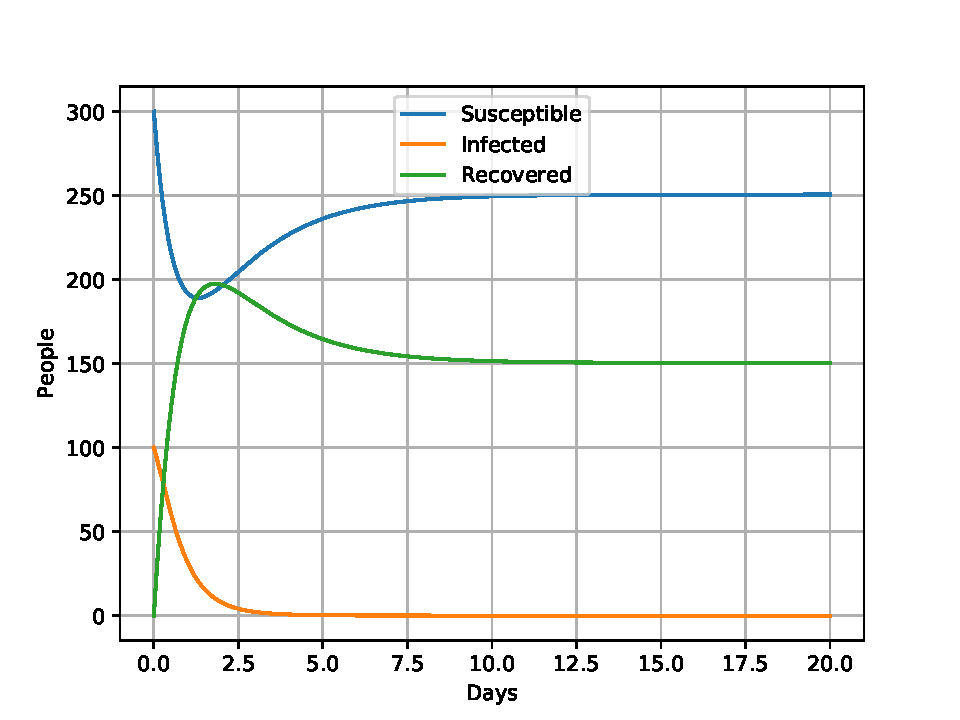
\includegraphics[scale=0.56]{../plots/opp_e_fd.pdf}
	\caption{fyll inn}
	%Label gjør det enkelt å referere til ulike bilder.
	\label{opp_e2}
\end{figure}



\section{DISCUSSION}



\section{CONCLUTION}




%\newpage
\section{APPENDICES}
All the calculations were done using the programing language Julia. The programs used can be found at:
\url{}.
	
%\section{REFERENCES}
\begin{thebibliography}{9}
	\bibitem{lecture notes}
	Computational Physics, Lecture Notes Fall 2015, Morten Hjort-Jensen p. 419-424
\end{thebibliography}




%\begin{figure}[h!]
%	\centering 
%	%Scale angir størrelsen på bildet. Bildefilen må ligge i samme mappe som tex-filen. 
%	\includegraphics[scale=0.7]{opp2_7.pdf}
%	\caption{A plot of the entropy}
%	%Label gjør det enkelt å referere til ulike bilder.
%	\label{2.7}
%\end{figure}







	
	
	
	
	
	
	
	
	
	
	
	
	
	
	
\end{document}




